\documentclass[addpoints]{exam}

    \makeatletter % Lagfæring fyrir nýjar útgáfur af TeXLive
    \expandafter\providecommand\expandafter*\csname ver@framed.sty\endcsname
    {2003/07/21 v0.8a Simulated by exam}
    \makeatother
    
    \usepackage[top=2cm, bottom=2cm, left=1cm, right=1cm]{geometry}
    \usepackage[utf8]{inputenc}
    \usepackage[icelandic]{babel}
    \usepackage[T1]{fontenc}
    % \usepackage[sc]{mathpazo}
    \usepackage{helvet} \renewcommand\familydefault{\sfdefault}
    
    \usepackage[parfill]{parskip}
    \usepackage{tabularx, booktabs}
    \usepackage{multirow}
    \usepackage{multicol}
    \usepackage{graphicx, tikz}
    \usepackage{enumerate}
    \usepackage{amsmath, amsfonts, amssymb, amsthm}
    \usepackage{minted} %Minted and configuration
    \usepackage{afterpage}
    \usepackage{scrextend}
    
    \usepackage[pdftex,bookmarks=true,colorlinks=true,pdfauthor={Eirikur Ernir Thorsteinsson},linkcolor=blue,urlcolor=blue]{hyperref}
    
    \newmintedfile[cppfile]{cpp}{frame=lines, linenos=false}
    \newmintedfile[javafile]{java}{frame=lines, linenos=false}
    \newcommand{\eng}[1]{(e.\ \emph{#1})}

    \setcounter{secnumdepth}{-1} 
    \hyphenpenalty=5000
    
    \newcommand\blankpage{%
        \null
        \thispagestyle{empty}%
        \addtocounter{page}{-1}%
        }
    
    \usemintedstyle{default}
    \renewcommand{\theFancyVerbLine}{\sffamily \arabic{FancyVerbLine}}
    \author{}
    \date{}
    
    \footer{}{}{}
    
    \setcounter{secnumdepth}{-1} 
    
    \qformat{\large \textbf Spurning \thequestion \phantom{M}(\totalpoints \phantom{l}stig) \hfill}
    \renewcommand{\solutiontitle}{\noindent\textbf{Svar:}\par\noindent}
    \renewcommand{\points}{stig}
    \renewcommand{\questionshook}{\setlength{\itemsep}{0.5cm}}
    \hqword{Spurning:}
    \hpword{Stig í boði:}
    \hsword{Stig:}
    \htword{Samtals}
    
    \title{TÖL203G Tölvunarfræði 2 - final exam}
    \author{}
    \date{maí 2018}
    
    \pagestyle{headandfoot}
    \firstpageheader{TÖL203G}{Tölvunarfræði 2 - Final exam}{maí 2018}
    \firstpagefooter{}{Page. \thepage\ of \numpages}{}
    \runningfooter{}{Page. \thepage\ of \numpages}{}
    \setlength{\columnsep}{0.5cm}
    
    \changefontsizes{14pt}

\begin{document}

Fullt nafn: \vspace*{1mm} \hrule

\vspace{1cm}

\textbf{Leiðbeiningar:} This exam has \numquestions\ questions totalling \numpoints\ points.
Permissible materials are a calculator and one A4 page of notes.

The sheets will be scanned for grading. Please avoid light pencils, do not tear or crumple the sheets, and do not add or remove pages.

To answer multiple choice questions, use the table below. Carefully mark one option for each question. Points are not deducted for incorrect answers. 

To answer other questions, write within the provided area. If additional space is required, use the last pages of the exam. Other parts of the sheets, particularly the overleaf, will not be read.

The questions on this exam are not ordered by difficulty.

\begin{center}
	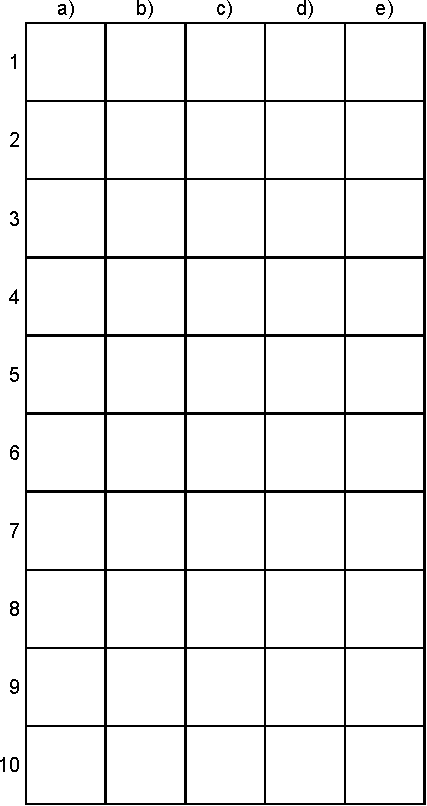
\includegraphics[width=0.4\linewidth]{Pics/svartafla}
\end{center}

\newpage

\begin{questions}

	\section{Multiple choice questions}

	\question[3]

	Which of the following is not an abstract data type?

	\begin{enumerate}[a)]
		\item Bag
		\item Stack
		\item Queue
        \item Singly linked list
        \item Graph
	\end{enumerate}

	\question[3]

	When the variable \texttt{i} is defined within a C++ function using the statement \texttt{int i = 0;}, its lifetime is\ldots

	\begin{enumerate}[a)]
		\item Primitive
		\item Static
		\item Dynamic
		\item Particular
		\item Automatic
	\end{enumerate}

	\question[3]

	A problematic C++ function is given. What is the problem?

	\begin{minted}[frame=lines]{cpp}
int* f( int a ) {
  int b = 2*a;
  return &b;
}
	\end{minted}
	
	\begin{enumerate}[a)]
		\item The function is syntactically incorrect
		\item The function does not return a pointer to an integer
		\item The function does not reserve memory for the variable \texttt{b}
		\item The function always returns \texttt{nullptr}
		\item The function returns a memory address from the stack
	\end{enumerate}

	\newpage

	\question[3]

	A C++ program is given.

	\cppfile[firstline=4, fontsize=\small, linenos=true]{Code/w14/Animals.cpp}

	What effect would it have to add the word \texttt{virtual} to the start of line 6, so that the method is defined as \texttt{virtual void move()}?

	\begin{enumerate}[a)]
		\item The program would write ``Dog runs!'' instead of ``Animal moves!''
		\item The program would write ``Animal moves!'' instead of ``Dog runs!''
		\item No effect, the program would still write ``Animal moves!''
		\item No effect, the program would still write ``Dog runs!''
		\item The program would not compile
	\end{enumerate}

	\question[3]

	If a queue is sensibly implemented using a singly linked list, of what order is the running time of insertion and deletion?

	\begin{enumerate}[a)]
		\item  $1$ (constant) insertion and deletion
		\item  $\log N$ insertion and deletion
		\item  $1$ insertion, $N$ deletion
		\item  $N$ insertion, $1$ deletion
		\item  $N$ insertion and deletion
	\end{enumerate}

	\newpage

	\question[3]

	Of what order is the running time of merge sort on an array with $N$ elements?

	\begin{multicols}{5}
		\begin{enumerate}[a)]
			\item $1$ (fasti)
			\item $\log N$
			\item $N$
			\item $N\log N$
			\item $N^2$
		\end{enumerate}
	\end{multicols}

	\question[3]

	$N$ keys are inserted in \emph{descending} order into a symbol table which is implemented using a simple binary tree. Of what order is the running time of a single lookup in the symbol table?

	\begin{multicols}{5}
		\begin{enumerate}[a)]
			\item $1$ (fasti)
			\item $\log N$
			\item $N$
			\item $N\log N$
			\item $N^2$
		\end{enumerate}
	\end{multicols}

	\question[3]

	$N$ keys are inserted in \emph{descending} order into a maximum priority queue which is implemented using a heap. Of what order is the total insertion time?

	\begin{multicols}{5}
		\begin{enumerate}[a)]
			\item $1$ (fasti)
			\item $\log N$
			\item $N$
			\item $N\log N$
			\item $N^2$
		\end{enumerate}
	\end{multicols}

	\question[3]

	Which of the following is a problem with using an adjacency matrix to implement a class which represents a graph?

	\begin{enumerate}[a)]
		\item The implementation is much more complicated than an implementation using adjacency lists
		\item It is difficult to see which vertices are adjacent using an adjacency matrix
		\item The memory usage is of the order of the number of vertices squared
		\item The memory usage is of the order of the number of edges squared
		\item Matrices are less CPU cache efficient than adjacency lists
	\end{enumerate}

	\question[3]

	Which of the following algorithms can be used to find the shortest path in an unweighted graph?

	\begin{enumerate}[a)]
		\item Prims's algorithm
		\item Kruskal's algorithm
		\item Depth-first search
		\item Breadth-first search
		\item Sierpinski's algorihtm
	\end{enumerate}

	\section{Written assignments}

	\question[5]

	Lists and arrays have a similar purpose in programming - storing elements which are accessible by indices. Name one advantage and one disadvantage of storing data in a singly linked list instead of an array.

	\makeemptybox{\stretch{1}}

	\question[5]
	Sedgewick and Wayne's quicksort implementation shuffles the collection before the actual algorithm starts. Name one advantage and one disadvantage of this arrangement.

	\makeemptybox{\stretch{1}}

	\newpage

	\question[5]

	The following table describes a hash function on the English alphabet:

	\begin{center}
		\scriptsize
		\begin{tabular}{l*{26}{c}}
			\toprule
			$x$    & A & B & C & D & E & F & G & H & I & J & K & L & M & N & O & P & Q & R & S & T & U & V & W & X & Y & Z \\
			\midrule
			$f(x)$ & 5 & 0 & 4 & 0 & 5 & 2 & 3 & 3 & 4 & 3 & 1 & 0 & 0 & 1 & 3 & 0 & 5 & 2 & 3 & 3 & 2 & 3 & 5 & 5 & 4 & 0 \\
			\bottomrule
		\end{tabular}
	\end{center}

	Scetch a separate chaining hash table which uses this hash function. Show its state after the keys T O L V U N A R F R A E D I have been inserted in order, assuming an initially empty table. Let the values be integers in increasing insertion order (zero-indexed).

	\makeemptybox{\stretch{1}}

	%	\question[5]

	%	Lýsið því hvernig árekstrar eru útkljáðir í “linear probing” hakkatöflu.

	%	\makeemptybox{\stretch{1}}

	\newpage

	\section{Programming assignments}

	\question[10]

	Write the method \texttt{removeOdds} in Java, which accepts a stack of integers as its input and removes from it all odd numbers, but does not otherwise change it.

	Method declaration: \texttt{void removeOdds(Stack<Integer> s)}

	\makeemptybox{\stretch{1}}

	\newpage

	\question[10]

	Write the C++ method \texttt{remove} which removes the node located at index \texttt{i} from a singly linked list. If \texttt{i} is 0, the first node is removed, if \texttt{i} is 1 the second node is removed, etc. Reference classes are in the appendix. 

	\texttt{0 <= i <= length -1} can be assumed when the method is run.

	Method declaration: \texttt{void remove(int i)}

	\makeemptybox{\stretch{1}}

	\newpage

	\question[10]

	Write binary search in Java. The method shall accept an array of ascending integers along with an integer key to be searched for. It shall return an array index where the search key is located. If the array does not contain the search key, the method shall return the integer -1.

	Method declaration: \texttt{int binarySearch(int[] a, int key)}

	\makeemptybox{\stretch{1}}

	\newpage

	\question[10]

	A partial implementation of a red-black tree is given in the appendix. Write a method in Java which accepts a node as its input and verifies whether the tree which has that node as its root is a legal red-black tree with respect to red-black coloring rules.

	Method declaration: \texttt{boolean isRedBlackTree(Node node)}

	\makeemptybox{\stretch{1}}

	\paragraph{Note:} It is not necessary to check whether the tree conforms to other rules about binary search trees.

	\newpage

	%	\question[10]

	%	Stefnd net án örvarása hafa þann eiginleika að fyrir þau má finna röðun \eng{topological ordering} svo að allir leggir netsins vísi í sömu átt. Sjá mynd í viðauka. Skrifið Java-aðferðina \texttt{ordering} sem tekur inn stefnt net (\texttt{Digraph}) og skilar slíkri röðun sem runu af hnútanúmerum (t.d. fylki eða \texttt{Iterable} hlut).

	%	\paragraph{Ábending:} Hægt er að nota aðferð sem líkist dýptarleit.

	\question

	\begin{parts}

		\part[5]

		Write the method \texttt{merge} in Java which accepts two queues of items sorted in ascending order as its input and returns the queue that results from merging the two queues in ascending order.

        Method signature: \texttt{static <Item extends Comparable<Item> > \\ Queue<Item> merge(Queue<Item> q1, Queue<Item> q2)}

        \makeemptybox{\stretch{1}}
        
        \newpage

		\part[10]

		Write a bottom-up merge sort implementation based on queues in Java, using the following approach: Split the $N$ elements of the collection into $N$ queues, each containing one element. Then repeatedly use the merging method from part a) until only one queue remains.

        Method signature: \texttt{void sort(Comparable[] a)}.
        
        \makeemptybox{\stretch{1}}

        \paragraph{Note:} You can assume that part a) was correctly implemented.

	\end{parts}


\end{questions}

\newpage

\section{Extra space}

The following extra space will be scanned. If it is used, reference it in the relevant question.

\makeemptybox{\stretch{1}}

\newpage

\makeemptybox{\stretch{1}}

\newpage

\section{Appendix}
The following APIs from \emph{Algorithms, 4th edition} are given:
\begin{center}
	%	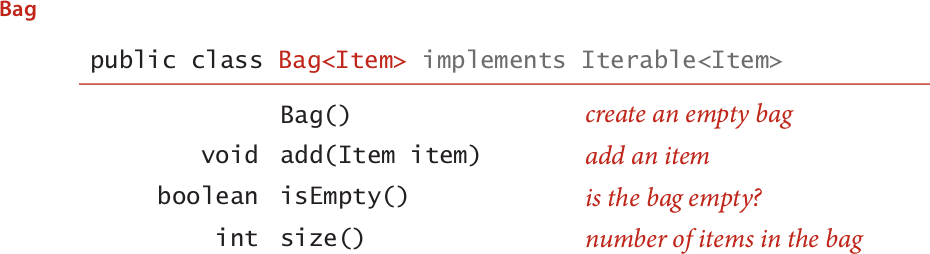
\includegraphics[width=0.8\textwidth]{Pics/API-Bag}

	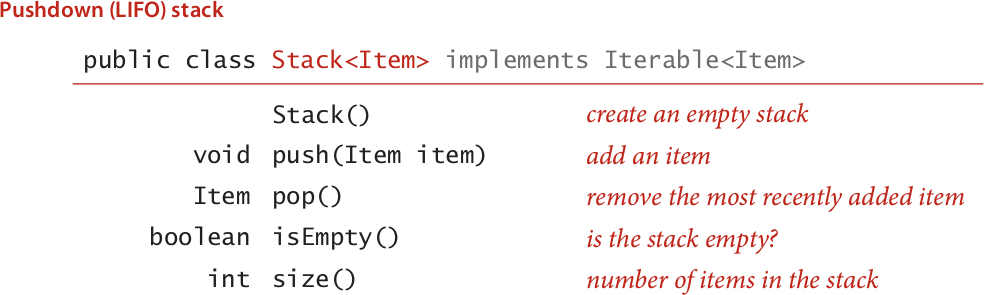
\includegraphics[width=0.7\textwidth]{Pics/API-Stack}

	\vspace{0.5cm}

	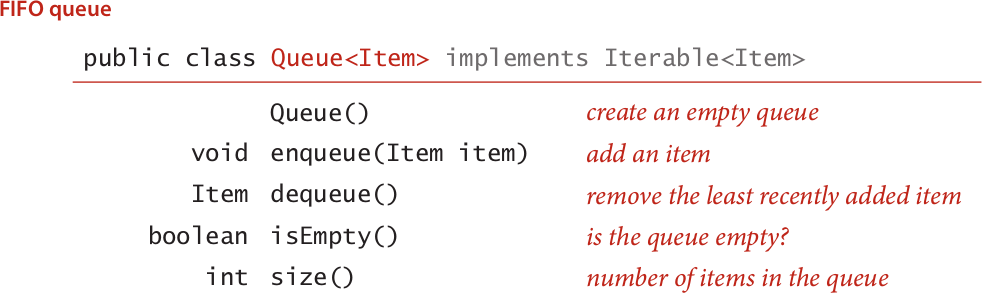
\includegraphics[width=0.7\textwidth]{Pics/API-Queue}

	%	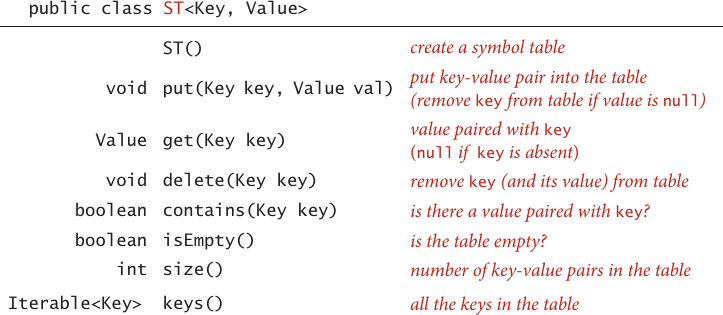
\includegraphics[width=0.8\textwidth]{Pics/API-ST}

	%	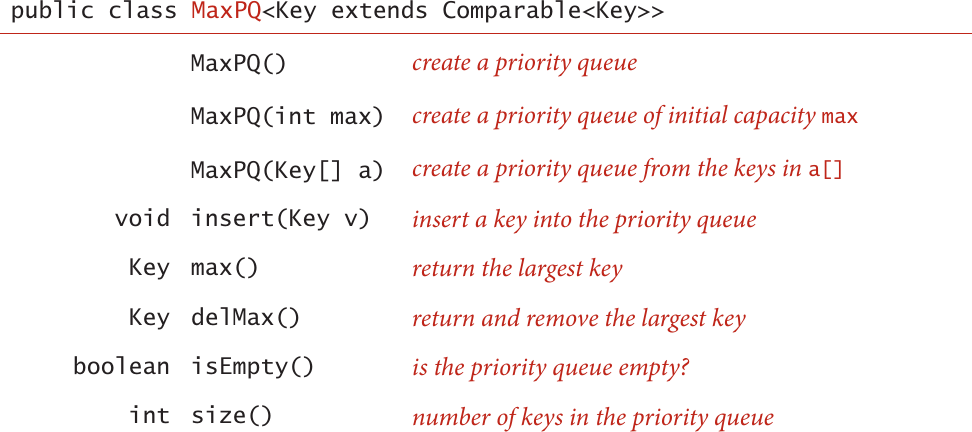
\includegraphics[width=0.8\textwidth]{Pics/API-MaxPQ}

	%	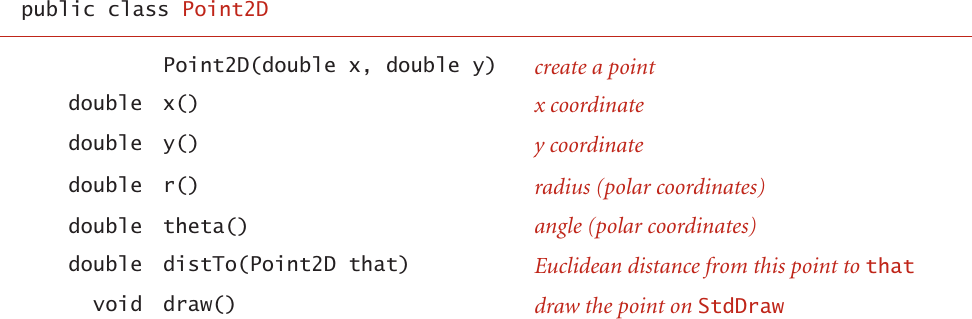
\includegraphics[width=0.8\textwidth]{Pics/API-Point2d}

	%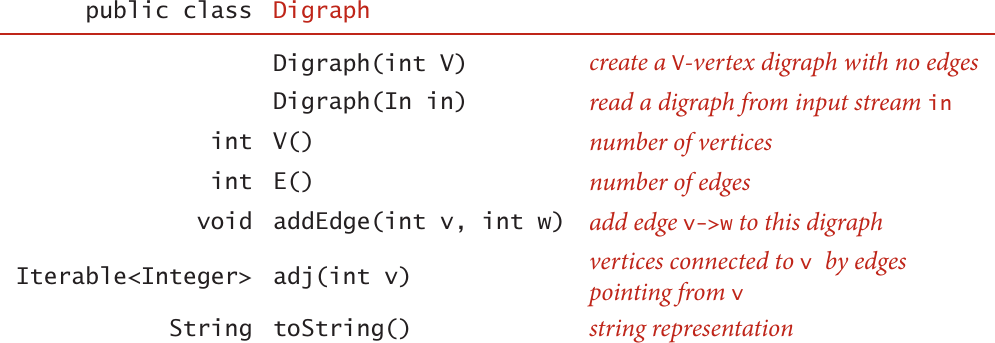
\includegraphics[width=0.8\textwidth]{Pics/API-Digraph}

	% 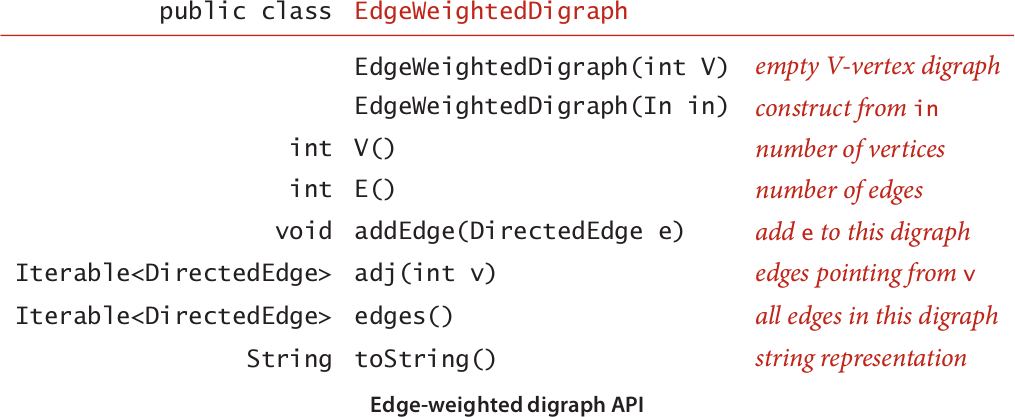
\includegraphics[width=0.8\textwidth]{Pics/API-EWDG}

	% \vspace{1cm}

	% 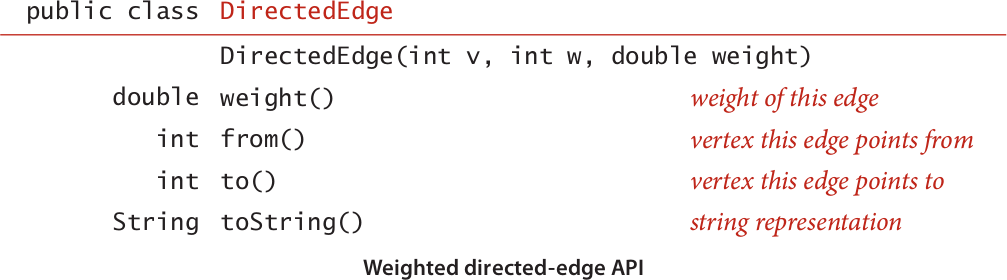
\includegraphics[width=0.8\textwidth]{Pics/API-DE}

	% \vspace{1cm}

    % 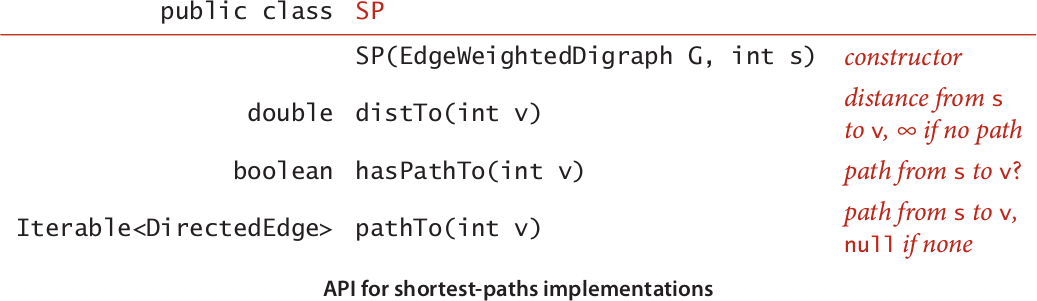
\includegraphics[width=0.8\textwidth]{Pics/API-SP}
    
\end{center}

	Classes for questions 15 og 17.
	\begin{multicols}{2}
		\cppfile[fontsize= \scriptsize]{Code/w14/LinkedList.cpp}

        \vspace{1cm}

		\javafile[fontsize= \scriptsize]{Code/w14/RedBlackTree.java}
	\end{multicols}

%%	Til vinstri: Stefnt rásalaust net. Til hægri: Röðunin 2 0 1 4 3 á netinu.
%%
%	\usetikzlibrary{arrows}
%	\begin{tikzpicture}
%		\tikzset{edge/.style = {->,> = latex'}}
%		\node (c1) at (2, 3) {2};
%		\node (d1) at (3, 2) {0};
%		\node (e1) at (3, 4) {1};
%		\node (f1) at (0, 3) {4};
%		\node (g1) at (0, 1) {3};
%
%		\draw[edge] (c1) to (f1);
%		\draw[edge] (c1) to (g1);
%		\draw[edge] (d1) to (e1);
%		\draw[edge] (e1) to (f1);
%
%		\node (c2) at (6, 1) {2};
%		\node (d2) at (6, 2) {0};
%		\node (e2) at (6, 3) {1};
%		\node (f2) at (6, 4) {4};
%		\node (g2) at (6, 5) {3};
%
%		\draw[edge] (c2) to[bend right=70] (f2);
%		\draw[edge] (c2) to[bend left=70] (g2);
%		\draw[edge] (d2) to (e2);
%		\draw[edge] (e2) to (f2);
%	\end{tikzpicture}

\end{document}